\chapter{Expanção em uma dimensão}
 Definido o método dos elementos finitos com a formulação de Galerkin, temos diferentes meios para resolver o problema. Anteriormente resolvemos uma equação diferencial usando elementos finitos com \textbf{equações lineares}. Discretizando o espaço em elementos de tamanho \textbf{h} e utilizando as técnicas de derivação e integração numérica utilizando polinômios de grau \textbf{p}, podemos utilizar a combinação desses métodos nos fornece aproximações com erros menores, para diferentes métodos.
 O método \textbf{p} utiliza um problema com um número de elementos fixo e para cada elemento usamos um  polinômio de grau \textbf{p} e verificamos a convergência do erro para cada grau desse polinômio. Temos o método \textbf{h} no qual fixamos o grau do polinômio e aumentamos o número de elementos, diminuindo o tamanho \textbf{h} de cada elemento.
 E o método espectral \textbf{hp} é a combinação de ambos os métodos anteriores, onde variamos o tamanho do elemento e o grau do polinômio para verificar a convergência do erro na obtenção de boas aproximações de uma função. 
 \section{Motivação do método hp}
 O método HP nos permite resolver problemas de geometrias complexas, no caso em uma dimensão casos com singularidades. Podemos verificar esse fenômenos em uma dimensão com a própria função de Runge anteriormente:
\begin{figure}[!h]
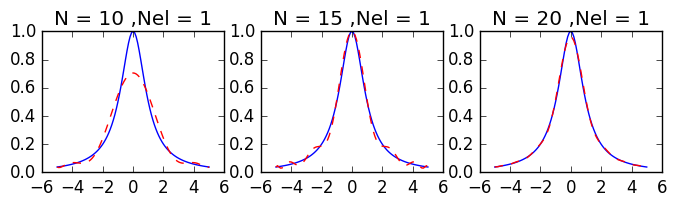
\includegraphics[width=0.6\textwidth, center ]{figuras/compara_metodo_n.png}
\caption{polinômio base de Lagrange para N  pontos em apenas um elemento}
\end{figure}
\\ Na figura acima vemos que para um problema subdividido em \emph{um} elemento, a aproximação acontece para um polinômio de lagrange de grau elevado, no caso anterior, n igual a 20. Porém  aumentando o número de elementos e tendo fixo o grau do polinômio, vemos que essa singularidade é contornada.

\begin{figure}[!b]
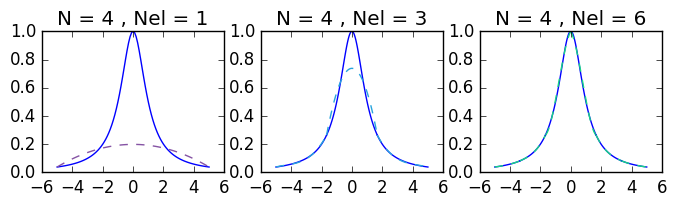
\includegraphics[width=0.6 \textwidth, center]{figuras/compara_metodo_n2.png}
\caption{Grau de polinômio fixo com diferentes números de elemento}
\end{figure}

\pagebreak
\section{Particionamento do domínio}
 Quando queremos solucionar um problema usando elementos , particionamos o seu domínio $\Omega$, definimos uma malha subdividida em $N_el$ elementos, de forma que não haja sobreposição dos mesmos.Matematicamente pode ser escrito como:\
\begin{equation}
 \Omega  = \bigcup^{Nel}_{e= 1} \Omega^e,\ onde\ \bigcap^{Nel}_{e= 1} \Omega^e = \varnothing
\end{equation}
Para um domínio $ \Omega = \{x\ | 0 \ <\ x\ <\ l  \}$, definímos sua malha por $Nel + 1$ pontos:
\begin{equation}
 0  = x_0 < x_1 < \ldots < x_{Nel - 1} < x_{Nel} = l
\end{equation}
Logo, o e-ésimo elemento é definido por:
\begin{equation}
 \Omega^e = \{x\ |\ x_{e-1}\ <\ x\ <\ x_{e}\ \}
\end{equation}
Ar
\begin{equation}
 \Omega^1 = \{x\ |\ x_{0}\ <\ x\ <\ x_{1}\ \}
\end{equation}



\section{Demonstração}
Frases: os modos globais podem ser representados em termos dos modos de expansão locais de cada elemento




omega padrão $\Omega_p$:
\begin{equation}
	\Omega_p = \{x\ |\ -1\ <\ x\ <\ 1\ \}
\end{equation}


mapeamento :
\begin{align}
x = \chi^e(\xi) = \frac{1-\xi}{2}x_{e-1}\ +\ \frac{1+\xi}{2}x_{e}\ ,\  \xi \in \Omega_{p}
\end{align}
inversa:
\begin{align}
\xi = (\chi^e) ^{-1}(x) = 2\ \frac{x - x_{e-1}}{x_{e} - x_{e-1}} - 1,\ x\ \in \   \Omega^e
\end{align}

lagrangiana
\begin{equation}
	h_i(x) = \prod_{k=1,k\ne i}^Q \frac{x - x_k}{x_i - x_k}
\end{equation}

\begin{align}
	 x = x
\end{align}



